
% Default to the notebook output style

    


% Inherit from the specified cell style.




    
\documentclass[11pt]{article}

    
    
    \usepackage[T1]{fontenc}
    % Nicer default font (+ math font) than Computer Modern for most use cases
    \usepackage{mathpazo}

    % Basic figure setup, for now with no caption control since it's done
    % automatically by Pandoc (which extracts ![](path) syntax from Markdown).
    \usepackage{graphicx}
    % We will generate all images so they have a width \maxwidth. This means
    % that they will get their normal width if they fit onto the page, but
    % are scaled down if they would overflow the margins.
    \makeatletter
    \def\maxwidth{\ifdim\Gin@nat@width>\linewidth\linewidth
    \else\Gin@nat@width\fi}
    \makeatother
    \let\Oldincludegraphics\includegraphics
    % Set max figure width to be 80% of text width, for now hardcoded.
    \renewcommand{\includegraphics}[1]{\Oldincludegraphics[width=.8\maxwidth]{#1}}
    % Ensure that by default, figures have no caption (until we provide a
    % proper Figure object with a Caption API and a way to capture that
    % in the conversion process - todo).
    \usepackage{caption}
    \DeclareCaptionLabelFormat{nolabel}{}
    \captionsetup{labelformat=nolabel}

    \usepackage{adjustbox} % Used to constrain images to a maximum size 
    \usepackage{xcolor} % Allow colors to be defined
    \usepackage{enumerate} % Needed for markdown enumerations to work
    \usepackage{geometry} % Used to adjust the document margins
    \usepackage{amsmath} % Equations
    \usepackage{amssymb} % Equations
    \usepackage{textcomp} % defines textquotesingle
    % Hack from http://tex.stackexchange.com/a/47451/13684:
    \AtBeginDocument{%
        \def\PYZsq{\textquotesingle}% Upright quotes in Pygmentized code
    }
    \usepackage{upquote} % Upright quotes for verbatim code
    \usepackage{eurosym} % defines \euro
    \usepackage[mathletters]{ucs} % Extended unicode (utf-8) support
    \usepackage[utf8x]{inputenc} % Allow utf-8 characters in the tex document
    \usepackage{fancyvrb} % verbatim replacement that allows latex
    \usepackage{grffile} % extends the file name processing of package graphics 
                         % to support a larger range 
    % The hyperref package gives us a pdf with properly built
    % internal navigation ('pdf bookmarks' for the table of contents,
    % internal cross-reference links, web links for URLs, etc.)
    \usepackage{hyperref}
    \usepackage{longtable} % longtable support required by pandoc >1.10
    \usepackage{booktabs}  % table support for pandoc > 1.12.2
    \usepackage[inline]{enumitem} % IRkernel/repr support (it uses the enumerate* environment)
    \usepackage[normalem]{ulem} % ulem is needed to support strikethroughs (\sout)
                                % normalem makes italics be italics, not underlines
    

    
    
    % Colors for the hyperref package
    \definecolor{urlcolor}{rgb}{0,.145,.698}
    \definecolor{linkcolor}{rgb}{.71,0.21,0.01}
    \definecolor{citecolor}{rgb}{.12,.54,.11}

    % ANSI colors
    \definecolor{ansi-black}{HTML}{3E424D}
    \definecolor{ansi-black-intense}{HTML}{282C36}
    \definecolor{ansi-red}{HTML}{E75C58}
    \definecolor{ansi-red-intense}{HTML}{B22B31}
    \definecolor{ansi-green}{HTML}{00A250}
    \definecolor{ansi-green-intense}{HTML}{007427}
    \definecolor{ansi-yellow}{HTML}{DDB62B}
    \definecolor{ansi-yellow-intense}{HTML}{B27D12}
    \definecolor{ansi-blue}{HTML}{208FFB}
    \definecolor{ansi-blue-intense}{HTML}{0065CA}
    \definecolor{ansi-magenta}{HTML}{D160C4}
    \definecolor{ansi-magenta-intense}{HTML}{A03196}
    \definecolor{ansi-cyan}{HTML}{60C6C8}
    \definecolor{ansi-cyan-intense}{HTML}{258F8F}
    \definecolor{ansi-white}{HTML}{C5C1B4}
    \definecolor{ansi-white-intense}{HTML}{A1A6B2}

    % commands and environments needed by pandoc snippets
    % extracted from the output of `pandoc -s`
    \providecommand{\tightlist}{%
      \setlength{\itemsep}{0pt}\setlength{\parskip}{0pt}}
    \DefineVerbatimEnvironment{Highlighting}{Verbatim}{commandchars=\\\{\}}
    % Add ',fontsize=\small' for more characters per line
    \newenvironment{Shaded}{}{}
    \newcommand{\KeywordTok}[1]{\textcolor[rgb]{0.00,0.44,0.13}{\textbf{{#1}}}}
    \newcommand{\DataTypeTok}[1]{\textcolor[rgb]{0.56,0.13,0.00}{{#1}}}
    \newcommand{\DecValTok}[1]{\textcolor[rgb]{0.25,0.63,0.44}{{#1}}}
    \newcommand{\BaseNTok}[1]{\textcolor[rgb]{0.25,0.63,0.44}{{#1}}}
    \newcommand{\FloatTok}[1]{\textcolor[rgb]{0.25,0.63,0.44}{{#1}}}
    \newcommand{\CharTok}[1]{\textcolor[rgb]{0.25,0.44,0.63}{{#1}}}
    \newcommand{\StringTok}[1]{\textcolor[rgb]{0.25,0.44,0.63}{{#1}}}
    \newcommand{\CommentTok}[1]{\textcolor[rgb]{0.38,0.63,0.69}{\textit{{#1}}}}
    \newcommand{\OtherTok}[1]{\textcolor[rgb]{0.00,0.44,0.13}{{#1}}}
    \newcommand{\AlertTok}[1]{\textcolor[rgb]{1.00,0.00,0.00}{\textbf{{#1}}}}
    \newcommand{\FunctionTok}[1]{\textcolor[rgb]{0.02,0.16,0.49}{{#1}}}
    \newcommand{\RegionMarkerTok}[1]{{#1}}
    \newcommand{\ErrorTok}[1]{\textcolor[rgb]{1.00,0.00,0.00}{\textbf{{#1}}}}
    \newcommand{\NormalTok}[1]{{#1}}
    
    % Additional commands for more recent versions of Pandoc
    \newcommand{\ConstantTok}[1]{\textcolor[rgb]{0.53,0.00,0.00}{{#1}}}
    \newcommand{\SpecialCharTok}[1]{\textcolor[rgb]{0.25,0.44,0.63}{{#1}}}
    \newcommand{\VerbatimStringTok}[1]{\textcolor[rgb]{0.25,0.44,0.63}{{#1}}}
    \newcommand{\SpecialStringTok}[1]{\textcolor[rgb]{0.73,0.40,0.53}{{#1}}}
    \newcommand{\ImportTok}[1]{{#1}}
    \newcommand{\DocumentationTok}[1]{\textcolor[rgb]{0.73,0.13,0.13}{\textit{{#1}}}}
    \newcommand{\AnnotationTok}[1]{\textcolor[rgb]{0.38,0.63,0.69}{\textbf{\textit{{#1}}}}}
    \newcommand{\CommentVarTok}[1]{\textcolor[rgb]{0.38,0.63,0.69}{\textbf{\textit{{#1}}}}}
    \newcommand{\VariableTok}[1]{\textcolor[rgb]{0.10,0.09,0.49}{{#1}}}
    \newcommand{\ControlFlowTok}[1]{\textcolor[rgb]{0.00,0.44,0.13}{\textbf{{#1}}}}
    \newcommand{\OperatorTok}[1]{\textcolor[rgb]{0.40,0.40,0.40}{{#1}}}
    \newcommand{\BuiltInTok}[1]{{#1}}
    \newcommand{\ExtensionTok}[1]{{#1}}
    \newcommand{\PreprocessorTok}[1]{\textcolor[rgb]{0.74,0.48,0.00}{{#1}}}
    \newcommand{\AttributeTok}[1]{\textcolor[rgb]{0.49,0.56,0.16}{{#1}}}
    \newcommand{\InformationTok}[1]{\textcolor[rgb]{0.38,0.63,0.69}{\textbf{\textit{{#1}}}}}
    \newcommand{\WarningTok}[1]{\textcolor[rgb]{0.38,0.63,0.69}{\textbf{\textit{{#1}}}}}
    
    
    % Define a nice break command that doesn't care if a line doesn't already
    % exist.
    \def\br{\hspace*{\fill} \\* }
    % Math Jax compatability definitions
    \def\gt{>}
    \def\lt{<}
    % Document parameters
    
\title{Chapter 1: Simple Harmonic Oscillators}

    
\date{7 and 10 September 2018}

    
\author{Nicolas Grisouard, nicolas.grisouard@physics.utoronto.ca}

    

    % Pygments definitions
    
\makeatletter
\def\PY@reset{\let\PY@it=\relax \let\PY@bf=\relax%
    \let\PY@ul=\relax \let\PY@tc=\relax%
    \let\PY@bc=\relax \let\PY@ff=\relax}
\def\PY@tok#1{\csname PY@tok@#1\endcsname}
\def\PY@toks#1+{\ifx\relax#1\empty\else%
    \PY@tok{#1}\expandafter\PY@toks\fi}
\def\PY@do#1{\PY@bc{\PY@tc{\PY@ul{%
    \PY@it{\PY@bf{\PY@ff{#1}}}}}}}
\def\PY#1#2{\PY@reset\PY@toks#1+\relax+\PY@do{#2}}

\expandafter\def\csname PY@tok@c\endcsname{\let\PY@it=\textit\def\PY@tc##1{\textcolor[rgb]{0.25,0.50,0.50}{##1}}}
\expandafter\def\csname PY@tok@kp\endcsname{\def\PY@tc##1{\textcolor[rgb]{0.00,0.50,0.00}{##1}}}
\expandafter\def\csname PY@tok@mb\endcsname{\def\PY@tc##1{\textcolor[rgb]{0.40,0.40,0.40}{##1}}}
\expandafter\def\csname PY@tok@sc\endcsname{\def\PY@tc##1{\textcolor[rgb]{0.73,0.13,0.13}{##1}}}
\expandafter\def\csname PY@tok@sx\endcsname{\def\PY@tc##1{\textcolor[rgb]{0.00,0.50,0.00}{##1}}}
\expandafter\def\csname PY@tok@nd\endcsname{\def\PY@tc##1{\textcolor[rgb]{0.67,0.13,1.00}{##1}}}
\expandafter\def\csname PY@tok@c1\endcsname{\let\PY@it=\textit\def\PY@tc##1{\textcolor[rgb]{0.25,0.50,0.50}{##1}}}
\expandafter\def\csname PY@tok@sr\endcsname{\def\PY@tc##1{\textcolor[rgb]{0.73,0.40,0.53}{##1}}}
\expandafter\def\csname PY@tok@ch\endcsname{\let\PY@it=\textit\def\PY@tc##1{\textcolor[rgb]{0.25,0.50,0.50}{##1}}}
\expandafter\def\csname PY@tok@sd\endcsname{\let\PY@it=\textit\def\PY@tc##1{\textcolor[rgb]{0.73,0.13,0.13}{##1}}}
\expandafter\def\csname PY@tok@sa\endcsname{\def\PY@tc##1{\textcolor[rgb]{0.73,0.13,0.13}{##1}}}
\expandafter\def\csname PY@tok@s\endcsname{\def\PY@tc##1{\textcolor[rgb]{0.73,0.13,0.13}{##1}}}
\expandafter\def\csname PY@tok@vi\endcsname{\def\PY@tc##1{\textcolor[rgb]{0.10,0.09,0.49}{##1}}}
\expandafter\def\csname PY@tok@no\endcsname{\def\PY@tc##1{\textcolor[rgb]{0.53,0.00,0.00}{##1}}}
\expandafter\def\csname PY@tok@mh\endcsname{\def\PY@tc##1{\textcolor[rgb]{0.40,0.40,0.40}{##1}}}
\expandafter\def\csname PY@tok@dl\endcsname{\def\PY@tc##1{\textcolor[rgb]{0.73,0.13,0.13}{##1}}}
\expandafter\def\csname PY@tok@gh\endcsname{\let\PY@bf=\textbf\def\PY@tc##1{\textcolor[rgb]{0.00,0.00,0.50}{##1}}}
\expandafter\def\csname PY@tok@si\endcsname{\let\PY@bf=\textbf\def\PY@tc##1{\textcolor[rgb]{0.73,0.40,0.53}{##1}}}
\expandafter\def\csname PY@tok@cp\endcsname{\def\PY@tc##1{\textcolor[rgb]{0.74,0.48,0.00}{##1}}}
\expandafter\def\csname PY@tok@il\endcsname{\def\PY@tc##1{\textcolor[rgb]{0.40,0.40,0.40}{##1}}}
\expandafter\def\csname PY@tok@gd\endcsname{\def\PY@tc##1{\textcolor[rgb]{0.63,0.00,0.00}{##1}}}
\expandafter\def\csname PY@tok@ni\endcsname{\let\PY@bf=\textbf\def\PY@tc##1{\textcolor[rgb]{0.60,0.60,0.60}{##1}}}
\expandafter\def\csname PY@tok@ne\endcsname{\let\PY@bf=\textbf\def\PY@tc##1{\textcolor[rgb]{0.82,0.25,0.23}{##1}}}
\expandafter\def\csname PY@tok@nt\endcsname{\let\PY@bf=\textbf\def\PY@tc##1{\textcolor[rgb]{0.00,0.50,0.00}{##1}}}
\expandafter\def\csname PY@tok@mo\endcsname{\def\PY@tc##1{\textcolor[rgb]{0.40,0.40,0.40}{##1}}}
\expandafter\def\csname PY@tok@vc\endcsname{\def\PY@tc##1{\textcolor[rgb]{0.10,0.09,0.49}{##1}}}
\expandafter\def\csname PY@tok@kd\endcsname{\let\PY@bf=\textbf\def\PY@tc##1{\textcolor[rgb]{0.00,0.50,0.00}{##1}}}
\expandafter\def\csname PY@tok@kt\endcsname{\def\PY@tc##1{\textcolor[rgb]{0.69,0.00,0.25}{##1}}}
\expandafter\def\csname PY@tok@nv\endcsname{\def\PY@tc##1{\textcolor[rgb]{0.10,0.09,0.49}{##1}}}
\expandafter\def\csname PY@tok@vm\endcsname{\def\PY@tc##1{\textcolor[rgb]{0.10,0.09,0.49}{##1}}}
\expandafter\def\csname PY@tok@mf\endcsname{\def\PY@tc##1{\textcolor[rgb]{0.40,0.40,0.40}{##1}}}
\expandafter\def\csname PY@tok@o\endcsname{\def\PY@tc##1{\textcolor[rgb]{0.40,0.40,0.40}{##1}}}
\expandafter\def\csname PY@tok@s2\endcsname{\def\PY@tc##1{\textcolor[rgb]{0.73,0.13,0.13}{##1}}}
\expandafter\def\csname PY@tok@cpf\endcsname{\let\PY@it=\textit\def\PY@tc##1{\textcolor[rgb]{0.25,0.50,0.50}{##1}}}
\expandafter\def\csname PY@tok@cs\endcsname{\let\PY@it=\textit\def\PY@tc##1{\textcolor[rgb]{0.25,0.50,0.50}{##1}}}
\expandafter\def\csname PY@tok@kc\endcsname{\let\PY@bf=\textbf\def\PY@tc##1{\textcolor[rgb]{0.00,0.50,0.00}{##1}}}
\expandafter\def\csname PY@tok@se\endcsname{\let\PY@bf=\textbf\def\PY@tc##1{\textcolor[rgb]{0.73,0.40,0.13}{##1}}}
\expandafter\def\csname PY@tok@go\endcsname{\def\PY@tc##1{\textcolor[rgb]{0.53,0.53,0.53}{##1}}}
\expandafter\def\csname PY@tok@cm\endcsname{\let\PY@it=\textit\def\PY@tc##1{\textcolor[rgb]{0.25,0.50,0.50}{##1}}}
\expandafter\def\csname PY@tok@gt\endcsname{\def\PY@tc##1{\textcolor[rgb]{0.00,0.27,0.87}{##1}}}
\expandafter\def\csname PY@tok@kr\endcsname{\let\PY@bf=\textbf\def\PY@tc##1{\textcolor[rgb]{0.00,0.50,0.00}{##1}}}
\expandafter\def\csname PY@tok@kn\endcsname{\let\PY@bf=\textbf\def\PY@tc##1{\textcolor[rgb]{0.00,0.50,0.00}{##1}}}
\expandafter\def\csname PY@tok@ge\endcsname{\let\PY@it=\textit}
\expandafter\def\csname PY@tok@gu\endcsname{\let\PY@bf=\textbf\def\PY@tc##1{\textcolor[rgb]{0.50,0.00,0.50}{##1}}}
\expandafter\def\csname PY@tok@s1\endcsname{\def\PY@tc##1{\textcolor[rgb]{0.73,0.13,0.13}{##1}}}
\expandafter\def\csname PY@tok@w\endcsname{\def\PY@tc##1{\textcolor[rgb]{0.73,0.73,0.73}{##1}}}
\expandafter\def\csname PY@tok@na\endcsname{\def\PY@tc##1{\textcolor[rgb]{0.49,0.56,0.16}{##1}}}
\expandafter\def\csname PY@tok@m\endcsname{\def\PY@tc##1{\textcolor[rgb]{0.40,0.40,0.40}{##1}}}
\expandafter\def\csname PY@tok@gi\endcsname{\def\PY@tc##1{\textcolor[rgb]{0.00,0.63,0.00}{##1}}}
\expandafter\def\csname PY@tok@nn\endcsname{\let\PY@bf=\textbf\def\PY@tc##1{\textcolor[rgb]{0.00,0.00,1.00}{##1}}}
\expandafter\def\csname PY@tok@nf\endcsname{\def\PY@tc##1{\textcolor[rgb]{0.00,0.00,1.00}{##1}}}
\expandafter\def\csname PY@tok@nc\endcsname{\let\PY@bf=\textbf\def\PY@tc##1{\textcolor[rgb]{0.00,0.00,1.00}{##1}}}
\expandafter\def\csname PY@tok@nl\endcsname{\def\PY@tc##1{\textcolor[rgb]{0.63,0.63,0.00}{##1}}}
\expandafter\def\csname PY@tok@nb\endcsname{\def\PY@tc##1{\textcolor[rgb]{0.00,0.50,0.00}{##1}}}
\expandafter\def\csname PY@tok@fm\endcsname{\def\PY@tc##1{\textcolor[rgb]{0.00,0.00,1.00}{##1}}}
\expandafter\def\csname PY@tok@vg\endcsname{\def\PY@tc##1{\textcolor[rgb]{0.10,0.09,0.49}{##1}}}
\expandafter\def\csname PY@tok@gp\endcsname{\let\PY@bf=\textbf\def\PY@tc##1{\textcolor[rgb]{0.00,0.00,0.50}{##1}}}
\expandafter\def\csname PY@tok@err\endcsname{\def\PY@bc##1{\setlength{\fboxsep}{0pt}\fcolorbox[rgb]{1.00,0.00,0.00}{1,1,1}{\strut ##1}}}
\expandafter\def\csname PY@tok@ss\endcsname{\def\PY@tc##1{\textcolor[rgb]{0.10,0.09,0.49}{##1}}}
\expandafter\def\csname PY@tok@gs\endcsname{\let\PY@bf=\textbf}
\expandafter\def\csname PY@tok@ow\endcsname{\let\PY@bf=\textbf\def\PY@tc##1{\textcolor[rgb]{0.67,0.13,1.00}{##1}}}
\expandafter\def\csname PY@tok@bp\endcsname{\def\PY@tc##1{\textcolor[rgb]{0.00,0.50,0.00}{##1}}}
\expandafter\def\csname PY@tok@gr\endcsname{\def\PY@tc##1{\textcolor[rgb]{1.00,0.00,0.00}{##1}}}
\expandafter\def\csname PY@tok@sh\endcsname{\def\PY@tc##1{\textcolor[rgb]{0.73,0.13,0.13}{##1}}}
\expandafter\def\csname PY@tok@k\endcsname{\let\PY@bf=\textbf\def\PY@tc##1{\textcolor[rgb]{0.00,0.50,0.00}{##1}}}
\expandafter\def\csname PY@tok@mi\endcsname{\def\PY@tc##1{\textcolor[rgb]{0.40,0.40,0.40}{##1}}}
\expandafter\def\csname PY@tok@sb\endcsname{\def\PY@tc##1{\textcolor[rgb]{0.73,0.13,0.13}{##1}}}

\def\PYZbs{\char`\\}
\def\PYZus{\char`\_}
\def\PYZob{\char`\{}
\def\PYZcb{\char`\}}
\def\PYZca{\char`\^}
\def\PYZam{\char`\&}
\def\PYZlt{\char`\<}
\def\PYZgt{\char`\>}
\def\PYZsh{\char`\#}
\def\PYZpc{\char`\%}
\def\PYZdl{\char`\$}
\def\PYZhy{\char`\-}
\def\PYZsq{\char`\'}
\def\PYZdq{\char`\"}
\def\PYZti{\char`\~}
% for compatibility with earlier versions
\def\PYZat{@}
\def\PYZlb{[}
\def\PYZrb{]}
\makeatother


    % Exact colors from NB
    \definecolor{incolor}{rgb}{0.0, 0.0, 0.5}
    \definecolor{outcolor}{rgb}{0.545, 0.0, 0.0}



    
    % Prevent overflowing lines due to hard-to-break entities
    \sloppy 
    % Setup hyperref package
    \hypersetup{
      breaklinks=true,  % so long urls are correctly broken across lines
      colorlinks=true,
      urlcolor=urlcolor,
      linkcolor=linkcolor,
      citecolor=citecolor,
      }
    % Slightly bigger margins than the latex defaults
    
    \geometry{verbose,tmargin=1in,bmargin=1in,lmargin=1in,rmargin=1in}
    
    

    \begin{document}
    
    
    \maketitle
    
    

    \newcommand{\rads}{~rad.s$^{-1}$}
\newcommand{\BV}{Brunt-V\"ais\"al\"a{} }
\newcommand{\bnabla}{\boldsymbol{\nabla}}
\newcommand{\eexp}[1]{\textsf{e}^{#1}}
\newcommand{\glm}[1]{\overline{#1}^L}
\newcommand{\psmom}[0]{\boldsymbol{\textsf{p}}}
\newcommand{\di}[0]{\textrm{d}}
\newcommand{\bs}[1]{\boldsymbol{#1}}
\newcommand{\ode}[2]{\frac{\di {#1}}{\di {#2}}}
\newcommand{\oden}[3]{\frac{\di^{#1} {#2}}{\di {#3}^{#1}}}
\newcommand{\odel}[2]{\di {#1}/\di {#2}}
\newcommand{\odeln}[3]{\di^{#1} {#2}/\di {#3}^{#1}}
\newcommand{\pde}[2]{\frac{\partial {#1}}{\partial {#2}}}
\newcommand{\pden}[3]{\frac{\partial^{#1} {#2}}{\partial {#3}^{#1}}}
\newcommand{\pdel}[2]{\partial_{#2} {#1}}
\newcommand{\pdenl}[3]{\partial^{#1}_{#3} {#2}}
\newcommand{\mde}[1]{\frac{\textrm{D} {#1}}{\textrm{D} t}}
\newcommand{\mdel}[1]{\textrm{D}_t {#1}}
\newcommand{\divr}[1]{\vec\nabla \cdot {#1}}
\newcommand{\divrb}[1]{\boldsymbol{\nabla} \cdot {#1}}
\newcommand{\grad}[1]{\vec \nabla {#1}}
\newcommand{\gradb}[1]{\boldsymbol\nabla {#1}}
\newcommand{\curl}[1]{\vec\nabla \times {#1}}
\newcommand{\curlb}[1]{\boldsymbol{\nabla}\times\boldsymbol{#1}}
\newcommand{\lapl}[0]{\vec\nabla^2}
\newcommand{\laplb}[0]{\boldsymbol{\nabla}^2}
\newcommand{\cplxi}[0]{\mathrm i}
\newcommand{\unit}[1]{\mathbf{\hat{#1}}}
\newcommand{\red}[1]{\textcolor{red}{#1}}
\newcommand{\blue}[1]{\textcolor{blue}{#1}}
\newcommand{\mage}[1]{\textcolor{magenta}{#1}}\DefineVerbatimEnvironment{Verbatim}{Verbatim}{fontsize=\scriptsize}

    \begin{Verbatim}[commandchars=\\\{\}]
{\color{incolor}In [{\color{incolor}1}]:} \PY{k+kn}{from} \PY{n+nn}{IPython}\PY{n+nn}{.}\PY{n+nn}{display} \PY{k}{import} \PY{n}{Image}\PY{p}{,} \PY{n}{display}
\end{Verbatim}


    \emph{{[}Book: chapter 1{]}}

This first chapter should be brief, a reminder of things you have seen
before (and if not, well, it's not that hard). I will mostly forcus on a
mass, oscillating because attached to a spring. Although very simple,
this system encapsulates many features that we will see throughout the
class. In particular, a second derivative will appear, and second
derivatives are all that this half-term is about.

All framed equations should be memorized.

    \hypertarget{expectations}{%
\section{Expectations}\label{expectations}}

I will have one of these sections at the beginning of each chapter. They
encapsulate what I am hoping to convey, and are usually divided into
three sub-sections/imperatives: ``Remember'' (the stuff I ask you to
remember), ``Understand'' (no need to memorize any of it, but you should
be able to read orit or mentally represent it to yourself easily),
``Create and apply'' (what types of exercises you should be able to
solve).

So, for this chapter:

    \hypertarget{remember}{%
\subsection{Remember}\label{remember}}

\begin{itemize}
\tightlist
\item
  Hooke's law.
\item
  The simple harmonic oscillator (SHO) equation,
  \(\ddot x + \omega^2 x = 0\).
\item
  For the mass-spring system, what each symbol above represents
  (acceleration, angular frequency, position, respectively).
\item
  For the mass-spring system, \(\omega^2 = k/m\).
\item
  How \(\omega\) (the angular frequency), \(\nu\) (the frequency) and
  \(T\) (the oscillation period) are related, and the units of each.
\item
  Solutions to the SHO are in the form of \(A\sin(\omega t + \phi)\),
  \(A\cos(\omega t + \phi)\), \(A_1\sin(\omega t) + A_2\cos(\omega t)\)
  or any linear combination of these.
\item
  That the three general solution forms above are equivalent, and can be
  turned into one another.
\item
  That the energy is proportional to the square of the amplitude.
\item
  That energies oscillate at twice the frequency of that of the position
  and velocity.
\end{itemize}

    \hypertarget{understand}{%
\subsection{Understand}\label{understand}}

\begin{itemize}
\tightlist
\item
  What the linear regime means.
\item
  How the SHO equation is assembled for the mass-spring system, and for
  the LC circuit.
\item
  How the general solution forms above are mathematical representations
  of the motion (or charge, etc.) or the physical system.
\item
  What the \(A\)'s and \(\phi\) above represent physically.
\end{itemize}

    \hypertarget{create-and-apply}{%
\subsection{Create and apply}\label{create-and-apply}}

\begin{itemize}
\tightlist
\item
  Turn one general solution form above into another, with the help of a
  trigonometric identity cheat sheet.
\item
  Do quick unit checks as a safeguard against algebra errors.
\item
  From a set of two initial conditions (e.g.~initial position
  \textbf{and} initial velocity, for the mass-spring system), how to
  compute the complete evolution of the system.
\end{itemize}

    \hypertarget{equations-of-motion}{%
\section{Equations of motion}\label{equations-of-motion}}

Consider the spring-mass system in fig. 1. An ideal spring (that is, a
weightless, dissipationless spring) of stiffess \(k > 0\) {[}in
N.m\(^{-1}\), or kg.s\(^{-2}\){]}, attached to a fixed wall on one end,
and an objet of mass \(m\) {[}kg{]} on the other.

\begin{figure}
\centering
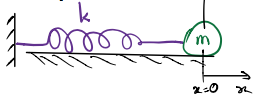
\includegraphics{SpringMass.png}
\caption{Fig. 1: Basic spring-mass system, with \(k\) the stiffness of
the spring and \(m\) the mass of the object.}
\end{figure}

Let \(x\) be the position of the centre of mass of the object. \(x=0\)
at rest, \(x\neq 0\) otherwise. Let's also assume the mass can slide on
the surface without friction, and that the spring is ``perfect'' (that
is, weightless and can oscillate without dissipation).

    We now pull the mass to position \(x = x_0 \neq 0\) and hold it there.
If \(x_0\) is ``not too big'', the spring will not deform or break. In
this case, the force of the spring on the mass is (Hooke's law)
\[ \Large \boxed{F = -kx_0.} \]

\begin{itemize}
\item
  The negative sign mean that the force is a \textbf{restoring force}
  (tends to bring back to origin).
\item
  \(k\) being constant, the force is proportional to the distance from
  rest state.
\end{itemize}

    For a Flash animation of Hooke's law, follow this link:

https://faraday.physics.utoronto.ca/GeneralInterest/Harrison/Flash/ClassMechanics/HookesLaw/HookesLaw.html

    This behaviour could define what ``linear'' means in physics. Any system
for which a state of rest can be defined will respond linearly
(``proportionnally'') to weak disturbances or forces.

\begin{figure}
\centering
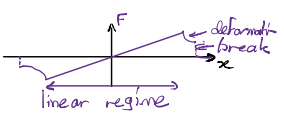
\includegraphics{Linear.png}
\caption{Fig. 2: Illustration of what linear behavious means.}
\end{figure}

\textbf{PHY293A: 100\% linear physics.}

\emph{Note that fig. 2 is incorrect for the spring: is a spring is
compressed to the max, it simply stops compressing. For \(x\) too far in
the negative, the non-linear regime is a vertical line representing an
infinite force for too much compression.}

    Let us now release our spring. The motion of the object has to obey
Newton's second law, which constitutes an equation of motion.
\[ ma = F\ \Rightarrow\ m\ddot{x} = -kx, \] with \(a = \ddot{x}\) the
acceleration. The equation above is a \textbf{second-order Ordinary
Differential Equation (ODE)}.

\textbf{PHY293A: 99\% 2}\(^{nd}\)\textbf{-order derivatives.}

\emph{Note: in this class, a dot on top of a quantity denotes its time
derivative, and time derivative only:}
\[ \dot{x} = \ode{x}t = v, \ \textrm{and}\ \ddot x = \oden{2}{x}{t} = a \]
\emph{It cannot denote, e.g., a spatial derivative, and e.g. \(\dot k\)
makes no sense because it is a constant.}

    \hypertarget{solutions}{%
\section{Solutions}\label{solutions}}

Let
\[\boxed{ \large \omega^2 = \frac{k}{m} \ \Rightarrow \ \ddot{x} + \omega^2 x = 0.} \]

    \(\omega\) is called the \emph{angular frequency}. Because \(k\) is in
kg.s\(^{-1}\) and \(m\) is in kg, \(\omega\) is in s\(^{-1}\) in SI
units. In many cases, people prefer to refer to the \emph{frequency}
(just frequency), as a measure of how many cycles per seconds there are.
Frequency \(\nu\) and angular frequency \(\omega\) are related via
\(\omega = 2\pi \nu\). Because one full cycle corresponds to \(2\pi\)
radians, many people prefer to refer to the units of \(\omega\) as
rad.s\(^{-1}\), and those of frequency as cycles.s\(^{-1}\), or Hz. It
makes it less confusing but not SI compliant (both cycles and radiants
have SI units of 1). In the context of this class, you are expected to
quote angular frequencies in rad.s\(^{-1}\) and frequencies in Hz, and
know which one is which.

    The solution of the framed equation above is
\[ x = A\cos(\omega t + \phi), \] with \(A\) the \emph{amplitude} of the
oscillation and \(\phi\) a \emph{phase}, both to be determined.

Note that because \(\cos(a+b) = \cos{a}\cos{b} - \sin{a}\sin{b}\), the
solution can also be written
\(x = A_1\cos(\omega t) + A_2\sin(\omega t)\), with \(A_1\) and \(A_2\)
now to be determined. My derivation could be done in these terms, but I
will stick to the first form of the solution.

    \begin{center}\rule{0.5\linewidth}{\linethickness}\end{center}

\emph{End of 09/07 lecture, beginning of 09/10 lecture.}

\begin{center}\rule{0.5\linewidth}{\linethickness}\end{center}

    We want to determine two parameters, \(A\) and \(\phi\). Therefore, we
need two pieces of information. We always have two \emph{initial
conditions}. For example, we can start with a ``clamped-mass'' kind of
initial condition:

\begin{enumerate}
\def\labelenumi{\arabic{enumi}.}
\item
  initially (at \(t=0\)), the position was \(x(t=0) = x_0\) and
\item
  we are holding the mass still (\(v(t=0)=0\)).
\end{enumerate}

The velocity is \[ v = \dot x = -A\omega\sin(\omega t + \phi). \]
Therefore, at \(t=0\),
\[ x(t=0) = x_0 = A\cos(\phi)\quad \textrm{and}\quad v(t=0) = 0 = -A\omega\sin(\phi). \]

    According to the second equation, either \(A =0\) or \(\phi=0\) or
\(\pi\). But \(A\neq0\), unless \(x_0 = 0\) (first eqn.). Therefore,
either \(\phi = 0\) and \(A=x_0\), or \(\phi = \pi\) and \(A = -x_0\).
Mathematically, both are correct because strictly equivalent. However,
\(A>0\) by definition in this class, and therefore, it is the sign of
\(x_0\) that determines which option is correct.

    Thus, \(x(t) = x_0\cos(\omega t)\). Let us plot this (numerical values
taken from the worked example of the book, page 9, except for the
initial velocity which is zero).

    \begin{Verbatim}[commandchars=\\\{\}]
{\color{incolor}In [{\color{incolor}2}]:} \PY{k+kn}{from} \PY{n+nn}{numpy} \PY{k}{import} \PY{n}{cos}\PY{p}{,} \PY{n}{sin}\PY{p}{,} \PY{n}{sqrt}\PY{p}{,} \PY{n}{linspace}\PY{p}{,} \PY{n}{pi}
        
        \PY{c+c1}{\PYZsh{} fundamental parameters}
        \PY{n}{k} \PY{o}{=} \PY{l+m+mf}{180.}  \PY{c+c1}{\PYZsh{} stiffness [N/m, kg/(s**2)]}
        \PY{n}{m} \PY{o}{=} \PY{l+m+mf}{0.8}  \PY{c+c1}{\PYZsh{} mass of object [kg]}
        \PY{n}{x0} \PY{o}{=} \PY{l+m+mf}{4e\PYZhy{}2}  \PY{c+c1}{\PYZsh{} initial position [m]}
        
        \PY{c+c1}{\PYZsh{} derived quantities}
        \PY{n}{omega} \PY{o}{=} \PY{n}{sqrt}\PY{p}{(}\PY{n}{k}\PY{o}{/}\PY{n}{m}\PY{p}{)}  \PY{c+c1}{\PYZsh{} angular frequency of the oscillation, [rad/s]}
        \PY{n}{T} \PY{o}{=} \PY{l+m+mi}{2}\PY{o}{*}\PY{n}{pi}\PY{o}{/}\PY{n}{omega}  \PY{c+c1}{\PYZsh{} period of oscillation [s]}
        \PY{n}{t} \PY{o}{=} \PY{n}{linspace}\PY{p}{(}\PY{l+m+mf}{0.}\PY{p}{,} \PY{l+m+mf}{0.6}\PY{p}{,} \PY{l+m+mi}{128}\PY{p}{)}  \PY{c+c1}{\PYZsh{} time array, from 0 to 0.6 s, 128 points}
        \PY{n}{x} \PY{o}{=} \PY{n}{x0}\PY{o}{*}\PY{n}{cos}\PY{p}{(}\PY{n}{omega}\PY{o}{*}\PY{n}{t}\PY{p}{)}  \PY{c+c1}{\PYZsh{} postion [m]}
        \PY{n}{v} \PY{o}{=} \PY{o}{\PYZhy{}}\PY{n}{x0}\PY{o}{*}\PY{n}{omega}\PY{o}{*}\PY{n}{sin}\PY{p}{(}\PY{n}{omega}\PY{o}{*}\PY{n}{t}\PY{p}{)}
\end{Verbatim}


    \begin{Verbatim}[commandchars=\\\{\}]
{\color{incolor}In [{\color{incolor}6}]:} \PY{c+c1}{\PYZsh{} let\PYZsq{}s plot}
        \PY{k+kn}{import} \PY{n+nn}{matplotlib}\PY{n+nn}{.}\PY{n+nn}{pyplot} \PY{k}{as} \PY{n+nn}{plt}
        \PY{k+kn}{from} \PY{n+nn}{matplotlib} \PY{k}{import} \PY{n}{interactive}
        \PY{n}{interactive}\PY{p}{(}\PY{k+kc}{False}\PY{p}{)}
        
        \PY{n}{ftsz}\PY{o}{=}\PY{l+m+mi}{13}  \PY{c+c1}{\PYZsh{} font size}
        \PY{n}{plt}\PY{o}{.}\PY{n}{figure}\PY{p}{(}\PY{p}{)}
        
        \PY{c+c1}{\PYZsh{} plotting the position x(t)}
        \PY{n}{ax1} \PY{o}{=} \PY{n}{plt}\PY{o}{.}\PY{n}{gca}\PY{p}{(}\PY{p}{)}
        \PY{n}{ax1}\PY{o}{.}\PY{n}{plot}\PY{p}{(}\PY{n}{t}\PY{p}{,} \PY{n}{x}\PY{p}{,} \PY{l+s+s1}{\PYZsq{}}\PY{l+s+s1}{b}\PY{l+s+s1}{\PYZsq{}}\PY{p}{)}  \PY{c+c1}{\PYZsh{} plotting the position x}
        \PY{n}{ax1}\PY{o}{.}\PY{n}{set\PYZus{}xlabel}\PY{p}{(}\PY{l+s+s1}{\PYZsq{}}\PY{l+s+s1}{time [s]}\PY{l+s+s1}{\PYZsq{}}\PY{p}{,} \PY{n}{fontsize}\PY{o}{=}\PY{n}{ftsz}\PY{p}{)} 
        \PY{n}{ax1}\PY{o}{.}\PY{n}{set\PYZus{}ylabel}\PY{p}{(}\PY{l+s+sa}{r}\PY{l+s+s1}{\PYZsq{}}\PY{l+s+s1}{position \PYZdl{}x\PYZdl{} [m]}\PY{l+s+s1}{\PYZsq{}}\PY{p}{,} \PY{n}{color}\PY{o}{=}\PY{l+s+s1}{\PYZsq{}}\PY{l+s+s1}{b}\PY{l+s+s1}{\PYZsq{}}\PY{p}{,} \PY{n}{fontsize}\PY{o}{=}\PY{n}{ftsz}\PY{p}{)}
        \PY{n}{ax1}\PY{o}{.}\PY{n}{tick\PYZus{}params}\PY{p}{(}\PY{l+s+s1}{\PYZsq{}}\PY{l+s+s1}{y}\PY{l+s+s1}{\PYZsq{}}\PY{p}{,} \PY{n}{colors}\PY{o}{=}\PY{l+s+s1}{\PYZsq{}}\PY{l+s+s1}{b}\PY{l+s+s1}{\PYZsq{}}\PY{p}{)}  \PY{c+c1}{\PYZsh{} color for y\PYZhy{}axis is blue}
        
        \PY{c+c1}{\PYZsh{} annotation to highlight the position amplitude}
        \PY{n}{ax1}\PY{o}{.}\PY{n}{axhline}\PY{p}{(}\PY{n}{x0}\PY{p}{,} \PY{n}{color}\PY{o}{=}\PY{l+s+s1}{\PYZsq{}}\PY{l+s+s1}{b}\PY{l+s+s1}{\PYZsq{}}\PY{p}{,} \PY{n}{linestyle}\PY{o}{=}\PY{l+s+s1}{\PYZsq{}}\PY{l+s+s1}{\PYZhy{}.}\PY{l+s+s1}{\PYZsq{}}\PY{p}{)}  \PY{c+c1}{\PYZsh{} the x=x0 mark}
        \PY{n}{ax1}\PY{o}{.}\PY{n}{text}\PY{p}{(}\PY{n}{T}\PY{o}{*}\PY{l+m+mf}{1.11}\PY{p}{,} \PY{n}{x0}\PY{p}{,} \PY{l+s+s1}{\PYZsq{}}\PY{l+s+s1}{\PYZdl{}x\PYZus{}0 = }\PY{l+s+si}{\PYZob{}0:1.0f\PYZcb{}}\PY{l+s+s1}{\PYZdl{} mm}\PY{l+s+s1}{\PYZsq{}}\PY{o}{.}\PY{n}{format}\PY{p}{(}\PY{n}{x0}\PY{o}{*}\PY{l+m+mi}{1000}\PY{p}{)}\PY{p}{,}
                 \PY{n}{verticalalignment}\PY{o}{=}\PY{l+s+s1}{\PYZsq{}}\PY{l+s+s1}{top}\PY{l+s+s1}{\PYZsq{}}\PY{p}{,} \PY{n}{horizontalalignment}\PY{o}{=}\PY{l+s+s1}{\PYZsq{}}\PY{l+s+s1}{left}\PY{l+s+s1}{\PYZsq{}}\PY{p}{,}
                 \PY{n}{color}\PY{o}{=}\PY{l+s+s1}{\PYZsq{}}\PY{l+s+s1}{b}\PY{l+s+s1}{\PYZsq{}}\PY{p}{)}
        
        \PY{n}{ax1}\PY{o}{.}\PY{n}{axhline}\PY{p}{(}\PY{l+m+mf}{0.}\PY{p}{,} \PY{n}{color}\PY{o}{=}\PY{l+s+s1}{\PYZsq{}}\PY{l+s+s1}{k}\PY{l+s+s1}{\PYZsq{}}\PY{p}{)}  \PY{c+c1}{\PYZsh{} draw the zero\PYZhy{}axis as horizontal line}
        
        \PY{c+c1}{\PYZsh{} plotting the velocity v(t)}
        \PY{n}{ax2} \PY{o}{=} \PY{n}{ax1}\PY{o}{.}\PY{n}{twinx}\PY{p}{(}\PY{p}{)}  \PY{c+c1}{\PYZsh{} creates another set of y\PYZhy{}axis on the right}
        \PY{n}{ax2}\PY{o}{.}\PY{n}{plot}\PY{p}{(}\PY{n}{t}\PY{p}{,} \PY{n}{v}\PY{p}{,} \PY{l+s+s1}{\PYZsq{}}\PY{l+s+s1}{r}\PY{l+s+s1}{\PYZsq{}}\PY{p}{)}  \PY{c+c1}{\PYZsh{} plotting the velocity v}
        \PY{n}{ax2}\PY{o}{.}\PY{n}{set\PYZus{}ylabel}\PY{p}{(}\PY{l+s+sa}{r}\PY{l+s+s1}{\PYZsq{}}\PY{l+s+s1}{velocity \PYZdl{}v\PYZdl{} [m/s]}\PY{l+s+s1}{\PYZsq{}}\PY{p}{,} \PY{n}{color}\PY{o}{=}\PY{l+s+s1}{\PYZsq{}}\PY{l+s+s1}{r}\PY{l+s+s1}{\PYZsq{}}\PY{p}{,} \PY{n}{fontsize}\PY{o}{=}\PY{n}{ftsz}\PY{p}{)}
        \PY{n}{ax2}\PY{o}{.}\PY{n}{tick\PYZus{}params}\PY{p}{(}\PY{n}{colors}\PY{o}{=}\PY{l+s+s1}{\PYZsq{}}\PY{l+s+s1}{r}\PY{l+s+s1}{\PYZsq{}}\PY{p}{)}  \PY{c+c1}{\PYZsh{} color for other y\PYZhy{}axis is red}
        \PY{n}{ax2}\PY{o}{.}\PY{n}{set\PYZus{}xlim}\PY{p}{(}\PY{p}{[}\PY{n}{t}\PY{o}{.}\PY{n}{min}\PY{p}{(}\PY{p}{)}\PY{p}{,} \PY{n}{t}\PY{o}{.}\PY{n}{max}\PY{p}{(}\PY{p}{)}\PY{p}{]}\PY{p}{)}
        
        \PY{c+c1}{\PYZsh{} annotation to highlight the velocity amplitude}
        \PY{n}{ax2}\PY{o}{.}\PY{n}{axhline}\PY{p}{(}\PY{o}{\PYZhy{}}\PY{n}{x0}\PY{o}{*}\PY{n}{omega}\PY{p}{,} \PY{n}{color}\PY{o}{=}\PY{l+s+s1}{\PYZsq{}}\PY{l+s+s1}{r}\PY{l+s+s1}{\PYZsq{}}\PY{p}{,} \PY{n}{linestyle}\PY{o}{=}\PY{l+s+s1}{\PYZsq{}}\PY{l+s+s1}{\PYZhy{}.}\PY{l+s+s1}{\PYZsq{}}\PY{p}{)}  \PY{c+c1}{\PYZsh{} the v=v0 mark}
        \PY{n}{ax2}\PY{o}{.}\PY{n}{text}\PY{p}{(}\PY{l+m+mf}{0.6}\PY{o}{*}\PY{n}{T}\PY{p}{,} \PY{o}{\PYZhy{}}\PY{n}{x0}\PY{o}{*}\PY{n}{omega}\PY{p}{,}
                 \PY{l+s+sa}{r}\PY{l+s+s1}{\PYZsq{}}\PY{l+s+s1}{\PYZdl{}|}\PY{l+s+s1}{\PYZbs{}}\PY{l+s+s1}{omega x\PYZus{}0| }\PY{l+s+s1}{\PYZbs{}}\PY{l+s+s1}{approx }\PY{l+s+si}{\PYZob{}0:1.1f\PYZcb{}}\PY{l+s+s1}{\PYZdl{} cm/s}\PY{l+s+s1}{\PYZsq{}}\PY{o}{.}\PY{n}{format}\PY{p}{(}\PY{n}{x0}\PY{o}{*}\PY{n}{omega}\PY{o}{*}\PY{l+m+mi}{100}\PY{p}{)}\PY{p}{,}
                 \PY{n}{verticalalignment}\PY{o}{=}\PY{l+s+s1}{\PYZsq{}}\PY{l+s+s1}{bottom}\PY{l+s+s1}{\PYZsq{}}\PY{p}{,} \PY{n}{horizontalalignment}\PY{o}{=}\PY{l+s+s1}{\PYZsq{}}\PY{l+s+s1}{left}\PY{l+s+s1}{\PYZsq{}}\PY{p}{,}
                 \PY{n}{color}\PY{o}{=}\PY{l+s+s1}{\PYZsq{}}\PY{l+s+s1}{r}\PY{l+s+s1}{\PYZsq{}}\PY{p}{)}
        
        \PY{c+c1}{\PYZsh{} annotation to highlight the period}
        \PY{n}{ax2}\PY{o}{.}\PY{n}{axvline}\PY{p}{(}\PY{n}{T}\PY{p}{,} \PY{n}{color}\PY{o}{=}\PY{l+s+s1}{\PYZsq{}}\PY{l+s+s1}{k}\PY{l+s+s1}{\PYZsq{}}\PY{p}{,} \PY{n}{linestyle}\PY{o}{=}\PY{l+s+s1}{\PYZsq{}}\PY{l+s+s1}{\PYZhy{}.}\PY{l+s+s1}{\PYZsq{}}\PY{p}{)}  \PY{c+c1}{\PYZsh{} the t=T mark}
        \PY{n}{ax2}\PY{o}{.}\PY{n}{annotate}\PY{p}{(}\PY{n}{s}\PY{o}{=}\PY{l+s+s1}{\PYZsq{}}\PY{l+s+s1}{\PYZsq{}}\PY{p}{,} \PY{n}{xy}\PY{o}{=}\PY{p}{(}\PY{l+m+mf}{0.}\PY{p}{,} \PY{l+m+mf}{4e\PYZhy{}2}\PY{p}{)}\PY{p}{,} \PY{n}{xytext}\PY{o}{=}\PY{p}{(}\PY{n}{T}\PY{p}{,} \PY{l+m+mf}{4e\PYZhy{}2}\PY{p}{)}\PY{p}{,}
                     \PY{n}{arrowprops}\PY{o}{=}\PY{n+nb}{dict}\PY{p}{(}\PY{n}{arrowstyle}\PY{o}{=}\PY{l+s+s1}{\PYZsq{}}\PY{l+s+s1}{\PYZlt{}|\PYZhy{}|\PYZgt{}}\PY{l+s+s1}{\PYZsq{}}\PY{p}{)}\PY{p}{)}  \PY{c+c1}{\PYZsh{} the double arrow}
        \PY{n}{ax2}\PY{o}{.}\PY{n}{text}\PY{p}{(}\PY{l+m+mf}{0.6}\PY{o}{*}\PY{n}{T}\PY{p}{,} \PY{l+m+mf}{4e\PYZhy{}2}\PY{p}{,} \PY{l+s+sa}{r}\PY{l+s+s1}{\PYZsq{}}\PY{l+s+s1}{\PYZdl{}T = 2}\PY{l+s+s1}{\PYZbs{}}\PY{l+s+s1}{pi/}\PY{l+s+s1}{\PYZbs{}}\PY{l+s+s1}{omega = }\PY{l+s+si}{\PYZob{}0:.2f\PYZcb{}}\PY{l+s+s1}{\PYZdl{} s}\PY{l+s+s1}{\PYZsq{}}\PY{o}{.}\PY{n}{format}\PY{p}{(}\PY{n}{T}\PY{p}{)}\PY{p}{,}
                 \PY{n}{verticalalignment}\PY{o}{=}\PY{l+s+s1}{\PYZsq{}}\PY{l+s+s1}{center}\PY{l+s+s1}{\PYZsq{}}\PY{p}{,} \PY{n}{horizontalalignment}\PY{o}{=}\PY{l+s+s1}{\PYZsq{}}\PY{l+s+s1}{center}\PY{l+s+s1}{\PYZsq{}}\PY{p}{,}
                 \PY{n}{backgroundcolor}\PY{o}{=}\PY{l+s+s1}{\PYZsq{}}\PY{l+s+s1}{w}\PY{l+s+s1}{\PYZsq{}}\PY{p}{,} \PY{n}{fontsize}\PY{o}{=}\PY{n}{ftsz}\PY{p}{)}
\end{Verbatim}


\begin{Verbatim}[commandchars=\\\{\}]
{\color{outcolor}Out[{\color{outcolor}6}]:} Text(0.251327,0.04,'\$T = 2\textbackslash{}\textbackslash{}pi/\textbackslash{}\textbackslash{}omega = 0.42\$ s')
\end{Verbatim}
            
    \begin{Verbatim}[commandchars=\\\{\}]
{\color{incolor}In [{\color{incolor}7}]:} \PY{n}{plt}\PY{o}{.}\PY{n}{show}\PY{p}{(}\PY{p}{)}
\end{Verbatim}


    \begin{center}
    \adjustimage{max size={0.9\linewidth}{0.9\paperheight}}{C01-SimpleHarmonicOscillator_files/C01-SimpleHarmonicOscillator_23_0.png}
    \end{center}
    { \hspace*{\fill} \\}
    
    \(T = 2\pi/\omega = 1/\nu\) is called the \emph{period} of the
oscillation, expressed in seconds.

    \emph{Suggested practise:}

\begin{itemize}
\item
  \emph{What happens to \(\omega\) if \(m\) or \(k\) increase? You can
  use the code above, but make sure you convince yourself that it makes
  physical sense.}
\item
  \emph{What if \(v(t=0) = v_0 \neq 0?\) Solve numerically with the
  values of King (worked example p.~9), and modify the code to plot it.
  Remove the annotations if they are annoying.}
\end{itemize}

    \begin{center}\rule{0.5\linewidth}{\linethickness}\end{center}

I will work out the second bullet point in detail here, but not in
class. The only difference with my previous example are the initial
conditions. We are still looking for a solution of the form
\(x = A\cos(\omega t + \phi)\). The velocity is
\(v = -A\omega\sin(\omega t + \phi)\).

Plugging the initial conditions for \(t=0\) yields \(x_0 = A \cos\phi\)
and \begin{align*}
    v_0 & = -A\omega\sin\phi \\
        & = -A\omega\sqrt{1-\cos^2\phi} \\
        & = -A\omega\sqrt{1-x_0^2/A^2} = -\omega\sqrt{A^2-x_0^2}.
\end{align*}

    If we square the last equation, we get
\[ v_0^2 - \omega^2(A^2 - x_0^2) = 0 \quad\Rightarrow\quad  A = \sqrt{x_0^2 + v_0^2/\omega^2}. \]
Note: technically, \(A\) should be \(\pm\) the result above.
Mathematically, we could choose \(A<0\), which would add or remove
\(\pi\) to the phase. However, an amplitude is always positive by
definition.

    The phase satisfies both \(\cos\phi = x_0/A\) and
\(\sin\phi = -v_0/(A\omega)\). At this point, the analytical approach
becomes cumbersome. Let us use the numerical values of King, p.9.:

    Let us use the numerical values of King, p.9.: \(m = 0.8\) kg,
\(k = 180\) N.m\(^{-1}\), therefore, \(\omega = 15\) rad.s\(^{-1}\). For
the initial conditions, \(x_0 = 4\) cm and \(v_0 = 0.5\) m.s\(^{-1}\),
and therefore, \(A \approx 5.21\) cm.

    Based on these numerical values, \(\cos\phi \approx 0.768\), meaning
\(\phi \approx \pm 39.8^\circ\), and \(\sin\phi \approx -0.640\),
meaning \(\phi \approx -39.8^\circ\) or \(220^\circ\). Therefore,
\(\phi \approx -39.8^\circ\).

    \begin{Verbatim}[commandchars=\\\{\}]
{\color{incolor}In [{\color{incolor}16}]:} \PY{k+kn}{from} \PY{n+nn}{numpy} \PY{k}{import} \PY{n}{arccos}\PY{p}{,} \PY{n}{arcsin}\PY{p}{,} \PY{n}{sqrt}
         \PY{n}{x0} \PY{o}{=} \PY{l+m+mf}{4e\PYZhy{}2}  \PY{c+c1}{\PYZsh{} 4 cm}
         \PY{n}{v0} \PY{o}{=} \PY{l+m+mf}{0.5}  \PY{c+c1}{\PYZsh{} m/s}
         \PY{n}{A} \PY{o}{=} \PY{n}{sqrt}\PY{p}{(}\PY{n}{x0}\PY{o}{*}\PY{o}{*}\PY{l+m+mi}{2} \PY{o}{+} \PY{n}{v0}\PY{o}{*}\PY{o}{*}\PY{l+m+mi}{2}\PY{o}{/}\PY{n}{omega}\PY{o}{*}\PY{o}{*}\PY{l+m+mi}{2}\PY{p}{)}
         \PY{n}{cos\PYZus{}of\PYZus{}phi} \PY{o}{=} \PY{n}{x0}\PY{o}{/}\PY{n}{A}
         \PY{n+nb}{print}\PY{p}{(}\PY{l+s+s1}{\PYZsq{}}\PY{l+s+s1}{phi = }\PY{l+s+si}{\PYZob{}0:.1f\PYZcb{}}\PY{l+s+s1}{ or }\PY{l+s+si}{\PYZob{}1:.1f\PYZcb{}}\PY{l+s+s1}{\PYZsq{}}\PY{o}{.}\PY{n}{format}\PY{p}{(}\PY{l+m+mi}{180}\PY{o}{*}\PY{n}{arccos}\PY{p}{(}\PY{n}{cos\PYZus{}of\PYZus{}phi}\PY{p}{)}\PY{o}{/}\PY{n}{pi}\PY{p}{,}
                                                 \PY{o}{\PYZhy{}}\PY{l+m+mi}{180}\PY{o}{*}\PY{n}{arccos}\PY{p}{(}\PY{n}{cos\PYZus{}of\PYZus{}phi}\PY{p}{)}\PY{o}{/}\PY{n}{pi}\PY{p}{)}\PY{p}{)}
\end{Verbatim}


    \begin{Verbatim}[commandchars=\\\{\}]
phi = 39.8 or -39.8

    \end{Verbatim}

    \begin{Verbatim}[commandchars=\\\{\}]
{\color{incolor}In [{\color{incolor}17}]:} \PY{n}{sin\PYZus{}of\PYZus{}phi} \PY{o}{=} \PY{o}{\PYZhy{}}\PY{n}{v0}\PY{o}{/}\PY{p}{(}\PY{n}{omega}\PY{o}{*}\PY{n}{A}\PY{p}{)}
         \PY{n+nb}{print}\PY{p}{(}\PY{l+s+s1}{\PYZsq{}}\PY{l+s+s1}{phi = }\PY{l+s+si}{\PYZob{}0:.1f\PYZcb{}}\PY{l+s+s1}{ or }\PY{l+s+si}{\PYZob{}1:.1f\PYZcb{}}\PY{l+s+s1}{\PYZsq{}}\PY{o}{.}\PY{n}{format}\PY{p}{(}\PY{l+m+mi}{180}\PY{o}{*}\PY{n}{arcsin}\PY{p}{(}\PY{n}{sin\PYZus{}of\PYZus{}phi}\PY{p}{)}\PY{o}{/}\PY{n}{pi}\PY{p}{,}
                                                 \PY{l+m+mi}{180}\PY{o}{\PYZhy{}}\PY{l+m+mi}{180}\PY{o}{*}\PY{n}{arcsin}\PY{p}{(}\PY{n}{sin\PYZus{}of\PYZus{}phi}\PY{p}{)}\PY{o}{/}\PY{n}{pi}\PY{p}{)}\PY{p}{)}
\end{Verbatim}


    \begin{Verbatim}[commandchars=\\\{\}]
phi = -39.8 or 219.8

    \end{Verbatim}

    \begin{Verbatim}[commandchars=\\\{\}]
{\color{incolor}In [{\color{incolor}18}]:} \PY{c+c1}{\PYZsh{} Let us plot}
         \PY{n}{phi} \PY{o}{=} \PY{o}{\PYZhy{}}\PY{l+m+mf}{39.8}\PY{o}{/}\PY{l+m+mi}{180}\PY{o}{*}\PY{n}{pi}
         \PY{n}{x} \PY{o}{=} \PY{n}{A}\PY{o}{*}\PY{n}{cos}\PY{p}{(}\PY{n}{omega}\PY{o}{*}\PY{n}{t} \PY{o}{+} \PY{n}{phi}\PY{p}{)}  \PY{c+c1}{\PYZsh{} position [m]}
         \PY{n}{v} \PY{o}{=} \PY{o}{\PYZhy{}}\PY{n}{A}\PY{o}{*}\PY{n}{omega}\PY{o}{*}\PY{n}{sin}\PY{p}{(}\PY{n}{omega}\PY{o}{*}\PY{n}{t} \PY{o}{+} \PY{n}{phi}\PY{p}{)}  \PY{c+c1}{\PYZsh{} velocity [m/s]}
\end{Verbatim}


    \begin{Verbatim}[commandchars=\\\{\}]
{\color{incolor}In [{\color{incolor}19}]:} \PY{c+c1}{\PYZsh{} let\PYZsq{}s plot}
         \PY{k+kn}{import} \PY{n+nn}{matplotlib}\PY{n+nn}{.}\PY{n+nn}{pyplot} \PY{k}{as} \PY{n+nn}{plt}
         
         \PY{n}{ftsz}\PY{o}{=}\PY{l+m+mi}{13}  \PY{c+c1}{\PYZsh{} font size}
         \PY{n}{plt}\PY{o}{.}\PY{n}{figure}\PY{p}{(}\PY{p}{)}
         
         \PY{c+c1}{\PYZsh{} plotting the position x(t)}
         \PY{n}{ax1} \PY{o}{=} \PY{n}{plt}\PY{o}{.}\PY{n}{gca}\PY{p}{(}\PY{p}{)}
         \PY{n}{ax1}\PY{o}{.}\PY{n}{plot}\PY{p}{(}\PY{n}{t}\PY{p}{,} \PY{n}{x}\PY{p}{,} \PY{l+s+s1}{\PYZsq{}}\PY{l+s+s1}{b}\PY{l+s+s1}{\PYZsq{}}\PY{p}{)}  \PY{c+c1}{\PYZsh{} plotting the position x}
         \PY{n}{ax1}\PY{o}{.}\PY{n}{set\PYZus{}xlabel}\PY{p}{(}\PY{l+s+s1}{\PYZsq{}}\PY{l+s+s1}{time [s]}\PY{l+s+s1}{\PYZsq{}}\PY{p}{,} \PY{n}{fontsize}\PY{o}{=}\PY{n}{ftsz}\PY{p}{)} 
         \PY{n}{ax1}\PY{o}{.}\PY{n}{set\PYZus{}ylabel}\PY{p}{(}\PY{l+s+sa}{r}\PY{l+s+s1}{\PYZsq{}}\PY{l+s+s1}{position \PYZdl{}x\PYZdl{} [m]}\PY{l+s+s1}{\PYZsq{}}\PY{p}{,} \PY{n}{color}\PY{o}{=}\PY{l+s+s1}{\PYZsq{}}\PY{l+s+s1}{b}\PY{l+s+s1}{\PYZsq{}}\PY{p}{,} \PY{n}{fontsize}\PY{o}{=}\PY{n}{ftsz}\PY{p}{)}
         \PY{n}{ax1}\PY{o}{.}\PY{n}{tick\PYZus{}params}\PY{p}{(}\PY{l+s+s1}{\PYZsq{}}\PY{l+s+s1}{y}\PY{l+s+s1}{\PYZsq{}}\PY{p}{,} \PY{n}{colors}\PY{o}{=}\PY{l+s+s1}{\PYZsq{}}\PY{l+s+s1}{b}\PY{l+s+s1}{\PYZsq{}}\PY{p}{)}  \PY{c+c1}{\PYZsh{} color for y\PYZhy{}axis is blue}
         
         \PY{n}{ax1}\PY{o}{.}\PY{n}{axhline}\PY{p}{(}\PY{l+m+mf}{0.}\PY{p}{,} \PY{n}{color}\PY{o}{=}\PY{l+s+s1}{\PYZsq{}}\PY{l+s+s1}{k}\PY{l+s+s1}{\PYZsq{}}\PY{p}{)}  \PY{c+c1}{\PYZsh{} draw the zero\PYZhy{}axis as horizontal line}
         
         \PY{c+c1}{\PYZsh{} plotting the velocity v(t)}
         \PY{n}{ax2} \PY{o}{=} \PY{n}{ax1}\PY{o}{.}\PY{n}{twinx}\PY{p}{(}\PY{p}{)}  \PY{c+c1}{\PYZsh{} creates another set of y\PYZhy{}axis on the right}
         \PY{n}{ax2}\PY{o}{.}\PY{n}{plot}\PY{p}{(}\PY{n}{t}\PY{p}{,} \PY{n}{v}\PY{p}{,} \PY{l+s+s1}{\PYZsq{}}\PY{l+s+s1}{r}\PY{l+s+s1}{\PYZsq{}}\PY{p}{)}  \PY{c+c1}{\PYZsh{} plotting the velocity v}
         \PY{n}{ax2}\PY{o}{.}\PY{n}{set\PYZus{}ylabel}\PY{p}{(}\PY{l+s+sa}{r}\PY{l+s+s1}{\PYZsq{}}\PY{l+s+s1}{velocity \PYZdl{}v\PYZdl{} [m/s]}\PY{l+s+s1}{\PYZsq{}}\PY{p}{,} \PY{n}{color}\PY{o}{=}\PY{l+s+s1}{\PYZsq{}}\PY{l+s+s1}{r}\PY{l+s+s1}{\PYZsq{}}\PY{p}{,} \PY{n}{fontsize}\PY{o}{=}\PY{n}{ftsz}\PY{p}{)}
         \PY{n}{ax2}\PY{o}{.}\PY{n}{tick\PYZus{}params}\PY{p}{(}\PY{n}{colors}\PY{o}{=}\PY{l+s+s1}{\PYZsq{}}\PY{l+s+s1}{r}\PY{l+s+s1}{\PYZsq{}}\PY{p}{)}  \PY{c+c1}{\PYZsh{} color for other y\PYZhy{}axis is red}
         \PY{n}{ax2}\PY{o}{.}\PY{n}{set\PYZus{}xlim}\PY{p}{(}\PY{p}{[}\PY{n}{t}\PY{o}{.}\PY{n}{min}\PY{p}{(}\PY{p}{)}\PY{p}{,} \PY{n}{t}\PY{o}{.}\PY{n}{max}\PY{p}{(}\PY{p}{)}\PY{p}{]}\PY{p}{)}
         
         \PY{n}{ax1}\PY{o}{.}\PY{n}{grid}\PY{p}{(}\PY{p}{)}
\end{Verbatim}


    \begin{Verbatim}[commandchars=\\\{\}]
{\color{incolor}In [{\color{incolor}20}]:} \PY{n}{plt}\PY{o}{.}\PY{n}{show}\PY{p}{(}\PY{p}{)}
\end{Verbatim}


    \begin{center}
    \adjustimage{max size={0.9\linewidth}{0.9\paperheight}}{C01-SimpleHarmonicOscillator_files/C01-SimpleHarmonicOscillator_35_0.png}
    \end{center}
    { \hspace*{\fill} \\}
    
    The figure above shows that with some positive initial velocity, the
mass keeps going in the positive direction for a little while. The
oscillation period remains the same however, and the curves above look
fundamentally the same as the ``clamped mass'' situation, earlier,
except for a shift in time.

    \hypertarget{energy-juggling}{%
\section{Energy Juggling}\label{energy-juggling}}

    Considering the energy is a powerful tool to solve many problems. SHOs
are no exception, because without dissipation, their total mechanical
energy stays the same forever.

You certainly remember that the kinetic energy (KE) \(K\) of an object
of mass \(m\) and velocity \(v\) is \[K = \frac12 m v^2.\] The only part
of the system that has KE is the mass, because the spring is ideal
(weightless).

    But what is the equivalent of the potential energy (PE), which I will
call \(U\)? When an object of mass \(m\) initially at rest is dropped in
vacuum and travels a distance \(h\), it KE is equal to \(mgh\), the PE
it had initially. Following this analogy, we measure \(U\) in our system
from a state when the KE is zero, i.e., when the spring is in a state of
maximal extension or compression. This time, it is the spring that
contains \(U\), not the mass. The spring packs all the potential for the
mass to gain KE. This is where the analogy with the dropped ball fails:
the PE that the ball had before being dropped was proportional to its
mass because the force that was going to set it in motion was the
gravitational force. Here, it is the force of the spring, which does not
care about the mass, or absence thereof, of the spring.

    So, back to our spring. The infinitesimal PE of an infinitesimally small
piece of spring located at position \(x'\) is related to the work
\(W = -\di U\) done when moving it by a distance \(\di x'\), following
\[ W = \vec F(x') \cdot \di \vec x' = -kx'\di x'. \]

The potential energy stored in the \emph{entire} spring whose length has
increased by \(x\) (the position of the mass) is therefore
\[ U = \int_0^x kx'\di x' = \frac12 kx^2. \]

    It is easy to check that the total mechanical energy is constant:
\[\boxed{ E = K + U = \frac12 mv^2 + \frac12 kx^2 = \frac12 k A^2 =  constant.} \]
Indeed, recall that we already computed \(x(t)\) and \(v(t)\). It is
simply a matter of substituting for them, and remembering that
\(\cos^2 + \sin^2 = 1\).

    Note that when I introduced this chapter, I mentioned that
considerations about energy conservation helped solve problems. Here, I
just did the opposite: I verified conservation of energy by solving the
problem first. King § 1.2.5 has a derivation that derives energy
conservation from Newton's 2\(^{nd}\) law, which you should definitely
check out.

    Back to the framed equation above: \textbf{the energy is proportional to
the square of the amplitude}, which is a very general statement about
oscillations. Remember it!

    \begin{Verbatim}[commandchars=\\\{\}]
{\color{incolor}In [{\color{incolor}24}]:} \PY{c+c1}{\PYZsh{} Let us plot this.}
         \PY{n}{K} \PY{o}{=} \PY{l+m+mf}{0.5}\PY{o}{*}\PY{n}{m}\PY{o}{*}\PY{n}{v}\PY{o}{*}\PY{o}{*}\PY{l+m+mi}{2}
         \PY{n}{U} \PY{o}{=} \PY{l+m+mf}{0.5}\PY{o}{*}\PY{n}{k}\PY{o}{*}\PY{n}{x}\PY{o}{*}\PY{o}{*}\PY{l+m+mi}{2}
         \PY{n}{E} \PY{o}{=} \PY{l+m+mf}{0.5}\PY{o}{*}\PY{n}{k}\PY{o}{*}\PY{n}{A}\PY{o}{*}\PY{o}{*}\PY{l+m+mi}{2}
\end{Verbatim}


    \begin{Verbatim}[commandchars=\\\{\}]
{\color{incolor}In [{\color{incolor}25}]:} \PY{c+c1}{\PYZsh{} Let us plot this.}
         \PY{n}{ftsz}\PY{o}{=}\PY{l+m+mi}{13}  \PY{c+c1}{\PYZsh{} font size}
         \PY{n}{plt}\PY{o}{.}\PY{n}{figure}\PY{p}{(}\PY{p}{)}
         
         \PY{n}{ax1} \PY{o}{=} \PY{n}{plt}\PY{o}{.}\PY{n}{gca}\PY{p}{(}\PY{p}{)}
         \PY{n}{ax1}\PY{o}{.}\PY{n}{plot}\PY{p}{(}\PY{n}{t}\PY{p}{,} \PY{n}{K}\PY{p}{,} \PY{l+s+s1}{\PYZsq{}}\PY{l+s+s1}{b}\PY{l+s+s1}{\PYZsq{}}\PY{p}{,} \PY{n}{label}\PY{o}{=}\PY{l+s+s1}{\PYZsq{}}\PY{l+s+s1}{\PYZdl{}K\PYZdl{}}\PY{l+s+s1}{\PYZsq{}}\PY{p}{)}  \PY{c+c1}{\PYZsh{} plotting the KE K}
         \PY{n}{ax1}\PY{o}{.}\PY{n}{plot}\PY{p}{(}\PY{n}{t}\PY{p}{,} \PY{n}{U}\PY{p}{,} \PY{l+s+s1}{\PYZsq{}}\PY{l+s+s1}{r\PYZhy{}\PYZhy{}}\PY{l+s+s1}{\PYZsq{}}\PY{p}{,} \PY{n}{label}\PY{o}{=}\PY{l+s+s1}{\PYZsq{}}\PY{l+s+s1}{\PYZdl{}U\PYZdl{}}\PY{l+s+s1}{\PYZsq{}}\PY{p}{)}  \PY{c+c1}{\PYZsh{} plotting the PE U}
         \PY{n}{ax1}\PY{o}{.}\PY{n}{legend}\PY{p}{(}\PY{p}{)}
         \PY{n}{ax1}\PY{o}{.}\PY{n}{set\PYZus{}xlabel}\PY{p}{(}\PY{l+s+s1}{\PYZsq{}}\PY{l+s+s1}{time [s]}\PY{l+s+s1}{\PYZsq{}}\PY{p}{,} \PY{n}{fontsize}\PY{o}{=}\PY{n}{ftsz}\PY{p}{)} 
         \PY{n}{ax1}\PY{o}{.}\PY{n}{set\PYZus{}ylabel}\PY{p}{(}\PY{l+s+sa}{r}\PY{l+s+s1}{\PYZsq{}}\PY{l+s+s1}{Energy [J, or kg.m\PYZdl{}\PYZca{}2\PYZdl{}.s\PYZdl{}\PYZca{}}\PY{l+s+s1}{\PYZob{}}\PY{l+s+s1}{\PYZhy{}2\PYZcb{}\PYZdl{}]}\PY{l+s+s1}{\PYZsq{}}\PY{p}{,} \PY{n}{color}\PY{o}{=}\PY{l+s+s1}{\PYZsq{}}\PY{l+s+s1}{b}\PY{l+s+s1}{\PYZsq{}}\PY{p}{,} \PY{n}{fontsize}\PY{o}{=}\PY{n}{ftsz}\PY{p}{)}
         
         \PY{c+c1}{\PYZsh{} annotation to highlight the total energy}
         \PY{n}{ax1}\PY{o}{.}\PY{n}{axhline}\PY{p}{(}\PY{n}{E}\PY{p}{,} \PY{n}{color}\PY{o}{=}\PY{l+s+s1}{\PYZsq{}}\PY{l+s+s1}{k}\PY{l+s+s1}{\PYZsq{}}\PY{p}{,} \PY{n}{linestyle}\PY{o}{=}\PY{l+s+s1}{\PYZsq{}}\PY{l+s+s1}{\PYZhy{}.}\PY{l+s+s1}{\PYZsq{}}\PY{p}{)}  \PY{c+c1}{\PYZsh{} total mechanical energy}
         \PY{n}{ax1}\PY{o}{.}\PY{n}{text}\PY{p}{(}\PY{n}{T}\PY{o}{*}\PY{l+m+mf}{1.11}\PY{p}{,} \PY{n}{E}\PY{o}{*}\PY{l+m+mf}{0.97}\PY{p}{,} \PY{l+s+s1}{\PYZsq{}}\PY{l+s+s1}{\PYZdl{}E = kA\PYZca{}2/2\PYZdl{}}\PY{l+s+s1}{\PYZsq{}}\PY{p}{,} \PY{n}{color}\PY{o}{=}\PY{l+s+s1}{\PYZsq{}}\PY{l+s+s1}{k}\PY{l+s+s1}{\PYZsq{}}\PY{p}{,}
                  \PY{n}{verticalalignment}\PY{o}{=}\PY{l+s+s1}{\PYZsq{}}\PY{l+s+s1}{top}\PY{l+s+s1}{\PYZsq{}}\PY{p}{,} \PY{n}{horizontalalignment}\PY{o}{=}\PY{l+s+s1}{\PYZsq{}}\PY{l+s+s1}{left}\PY{l+s+s1}{\PYZsq{}}\PY{p}{,}
                  \PY{n}{backgroundcolor}\PY{o}{=}\PY{l+s+s1}{\PYZsq{}}\PY{l+s+s1}{w}\PY{l+s+s1}{\PYZsq{}}\PY{p}{,} \PY{n}{fontsize}\PY{o}{=}\PY{n}{ftsz}\PY{p}{)}
         
         \PY{n}{ax1}\PY{o}{.}\PY{n}{axhline}\PY{p}{(}\PY{l+m+mf}{0.}\PY{p}{,} \PY{n}{color}\PY{o}{=}\PY{l+s+s1}{\PYZsq{}}\PY{l+s+s1}{k}\PY{l+s+s1}{\PYZsq{}}\PY{p}{)}  \PY{c+c1}{\PYZsh{} draw the zero\PYZhy{}axis as horizontal line}
         \PY{n}{ax1}\PY{o}{.}\PY{n}{set\PYZus{}xlim}\PY{p}{(}\PY{p}{[}\PY{n}{t}\PY{o}{.}\PY{n}{min}\PY{p}{(}\PY{p}{)}\PY{p}{,} \PY{n}{t}\PY{o}{.}\PY{n}{max}\PY{p}{(}\PY{p}{)}\PY{p}{]}\PY{p}{)}
         
         \PY{c+c1}{\PYZsh{} annotation to highlight the period}
         \PY{n}{ax1}\PY{o}{.}\PY{n}{axvline}\PY{p}{(}\PY{n}{T}\PY{p}{,} \PY{n}{color}\PY{o}{=}\PY{l+s+s1}{\PYZsq{}}\PY{l+s+s1}{k}\PY{l+s+s1}{\PYZsq{}}\PY{p}{,} \PY{n}{linestyle}\PY{o}{=}\PY{l+s+s1}{\PYZsq{}}\PY{l+s+s1}{\PYZhy{}.}\PY{l+s+s1}{\PYZsq{}}\PY{p}{)}  \PY{c+c1}{\PYZsh{} the t=T mark}
         \PY{n}{ax1}\PY{o}{.}\PY{n}{annotate}\PY{p}{(}\PY{n}{s}\PY{o}{=}\PY{l+s+s1}{\PYZsq{}}\PY{l+s+s1}{\PYZsq{}}\PY{p}{,} \PY{n}{xy}\PY{o}{=}\PY{p}{(}\PY{l+m+mf}{0.}\PY{p}{,} \PY{l+m+mf}{0.2}\PY{o}{*}\PY{n}{E}\PY{p}{)}\PY{p}{,} \PY{n}{xytext}\PY{o}{=}\PY{p}{(}\PY{n}{T}\PY{p}{,} \PY{l+m+mf}{0.2}\PY{o}{*}\PY{n}{E}\PY{p}{)}\PY{p}{,}
                      \PY{n}{arrowprops}\PY{o}{=}\PY{n+nb}{dict}\PY{p}{(}\PY{n}{arrowstyle}\PY{o}{=}\PY{l+s+s1}{\PYZsq{}}\PY{l+s+s1}{\PYZlt{}|\PYZhy{}|\PYZgt{}}\PY{l+s+s1}{\PYZsq{}}\PY{p}{)}\PY{p}{)}  \PY{c+c1}{\PYZsh{} the double arrow}
         \PY{n}{ax1}\PY{o}{.}\PY{n}{text}\PY{p}{(}\PY{n}{T}\PY{o}{/}\PY{l+m+mi}{2}\PY{p}{,} \PY{l+m+mf}{0.2}\PY{o}{*}\PY{n}{E}\PY{p}{,} \PY{l+s+sa}{r}\PY{l+s+s1}{\PYZsq{}}\PY{l+s+s1}{\PYZdl{}T = 2}\PY{l+s+s1}{\PYZbs{}}\PY{l+s+s1}{pi/}\PY{l+s+s1}{\PYZbs{}}\PY{l+s+s1}{omega }\PY{l+s+s1}{\PYZbs{}}\PY{l+s+s1}{approx }\PY{l+s+si}{\PYZob{}0:.2f\PYZcb{}}\PY{l+s+s1}{\PYZdl{} s}\PY{l+s+s1}{\PYZsq{}}\PY{o}{.}\PY{n}{format}\PY{p}{(}\PY{n}{T}\PY{p}{)}\PY{p}{,}
                  \PY{n}{verticalalignment}\PY{o}{=}\PY{l+s+s1}{\PYZsq{}}\PY{l+s+s1}{center}\PY{l+s+s1}{\PYZsq{}}\PY{p}{,} \PY{n}{horizontalalignment}\PY{o}{=}\PY{l+s+s1}{\PYZsq{}}\PY{l+s+s1}{center}\PY{l+s+s1}{\PYZsq{}}\PY{p}{,}
                  \PY{n}{backgroundcolor}\PY{o}{=}\PY{l+s+s1}{\PYZsq{}}\PY{l+s+s1}{w}\PY{l+s+s1}{\PYZsq{}}\PY{p}{,} \PY{n}{fontsize}\PY{o}{=}\PY{n}{ftsz}\PY{p}{)}
\end{Verbatim}


\begin{Verbatim}[commandchars=\\\{\}]
{\color{outcolor}Out[{\color{outcolor}25}]:} Text(0.20944,0.0488,'\$T = 2\textbackslash{}\textbackslash{}pi/\textbackslash{}\textbackslash{}omega \textbackslash{}\textbackslash{}approx 0.42\$ s')
\end{Verbatim}
            
    \begin{Verbatim}[commandchars=\\\{\}]
{\color{incolor}In [{\color{incolor}26}]:} \PY{n}{plt}\PY{o}{.}\PY{n}{show}\PY{p}{(}\PY{p}{)}
\end{Verbatim}


    \begin{center}
    \adjustimage{max size={0.9\linewidth}{0.9\paperheight}}{C01-SimpleHarmonicOscillator_files/C01-SimpleHarmonicOscillator_46_0.png}
    \end{center}
    { \hspace*{\fill} \\}
    
    Which makes sense: at maximum extension, \(K=0\) and \(U = kx_0^2/2\) is
maximum. When the mass passes by the rest position \(x=0\) at \(t=T/4\),
the velocity and therefore \(K\) are at their maxima, but the spring is
neither stretched or compressed and \(U=0\). Half a period later, the
spring is at its maximum compression (if initially stretched),
\(U = kx_0^2/2\) again, and the velocity is zero (\(K=0\) again).

Notice how I just described a \textbf{frequency doubling}: \(K\) and
\(U\) get back to their original values after \emph{half} a period. The
periodicity of \(K\) and \(U\) is twice that of \(x\) and \(v\), which
one can tell mathematically because
\(\sin^2(\omega t) = [1 - \cos(2\omega t)]/2\) and
\(\cos^2(\omega t) = [1 + \cos(2\omega t)]/2\). \textbf{Remember this!}

    \hypertarget{electrical-analogy-lc-circuit}{%
\section{Electrical Analogy: LC
Circuit}\label{electrical-analogy-lc-circuit}}

    \hypertarget{solutions}{%
\subsection{Solutions}\label{solutions}}

    The derivation we just did can be applied to countless systems. It could
be about small oscillations of a pendulum (King § 1.3), a horizontal
disk hanging from a tortional string, and many more. They all obey a
second-order ODE, and the different physics of each oscillator is
contained in the angular frequency \(\omega\). We illustrate this point
with an electric circuit consisting of a capacitor (capacitance \(C\))
and an inductor (inductance \(L\)) connected in series, with a switch
in-between (cf.~fig. 3). As for the spring, where we ignored all
frictional or dissipative processes, we ignore the resistance in the
circuit for now. But not to fear, young waver: it will take back its
rightful place in the next chapter.

    \begin{figure}
\centering
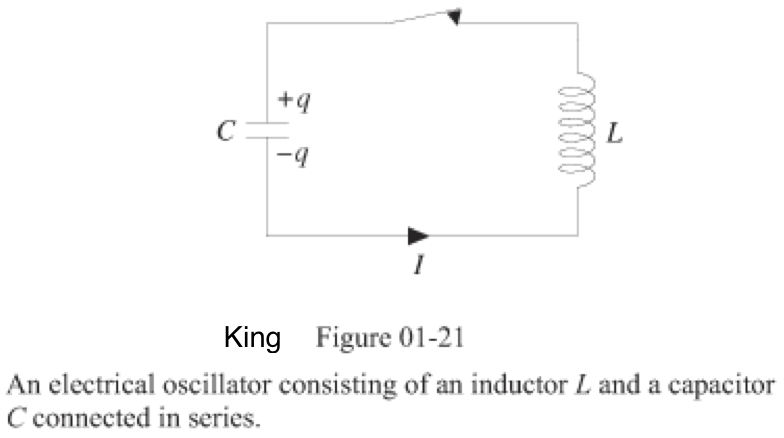
\includegraphics{LC_circuit.png}
\caption{Fig. 3}
\end{figure}

    Initial conditions:

\begin{enumerate}
\def\labelenumi{\arabic{enumi}.}
\item
  Switch is open, capacitor is charged to voltage \(V_C\). The charge in
  the capacitor is \(q = CV_C\).
\item
  Switch is open thus currrent \(I=\dot{q} = 0\).
\end{enumerate}

    We then close the switch. Current starts flowing, \(I = \dot q \neq 0\),
and the voltage accross \(L\) is \(V_L = L \dot I\). Therefore,
\[ \underbrace{V_L+V_C = 0}_{Kirchhof\!f's\ law} = L\dot I + \frac{q}C  = L\ddot q + \frac{q}C, \]
or, written in a now familiar form,
\[ \boxed{\ddot q + \omega^2 q = 0, \quad \textrm{with}\quad \omega^2 = 1/(LC).} \]

    Based on the few equations above, there is a one-to-one correspondence
between the mass+spring and the capacitor+inductor system. The capacitor
packs `potential energy' (actually, electrostatic energy) and relases it
as `kinetic energy' (actually, magnetic energy), which the inductor uses
to send electrons in the other direction and revert the sign of the
voltage. More specifically, the correspondance is:

    \begin{longtable}[]{@{}cc@{}}
\toprule
Mass+spring & LC circuit\tabularnewline
\midrule
\endhead
\(x\) & \(q\)\tabularnewline
\(v\) & \(I\)\tabularnewline
\(m\) & \(L\)\tabularnewline
\(k\) & \(1/C\)\tabularnewline
KE \(K = mv^2/2\) & Magnetic energy \(LI^2/2\)\tabularnewline
PE \(U = kx^2/2\) & Electrostatic energy \(CV_C^2/2\)\tabularnewline
\bottomrule
\end{longtable}


    % Add a bibliography block to the postdoc
    
    
    
    \end{document}
